\documentclass[tikz,border=12pt]{standalone}
\usepackage[T1]{fontenc}
\usepackage{mathpazo}
\usepackage{amsmath,amssymb}
\usetikzlibrary{arrows.meta, positioning, calc, fit, patterns, decorations.pathreplacing}

\definecolor{stblue}{HTML}{7B97AD}
\definecolor{rwgold}{HTML}{B8995E}
\definecolor{sage}{HTML}{7A9A7E}
\definecolor{dkbrown}{HTML}{3D3530}
\definecolor{wmgray}{HTML}{7B7067}
\definecolor{cream}{HTML}{F9F6F0}
\definecolor{border}{HTML}{D4C9B8}
\definecolor{terracotta}{HTML}{C47A6A}
\definecolor{lavender}{HTML}{907EA0}

\begin{document}
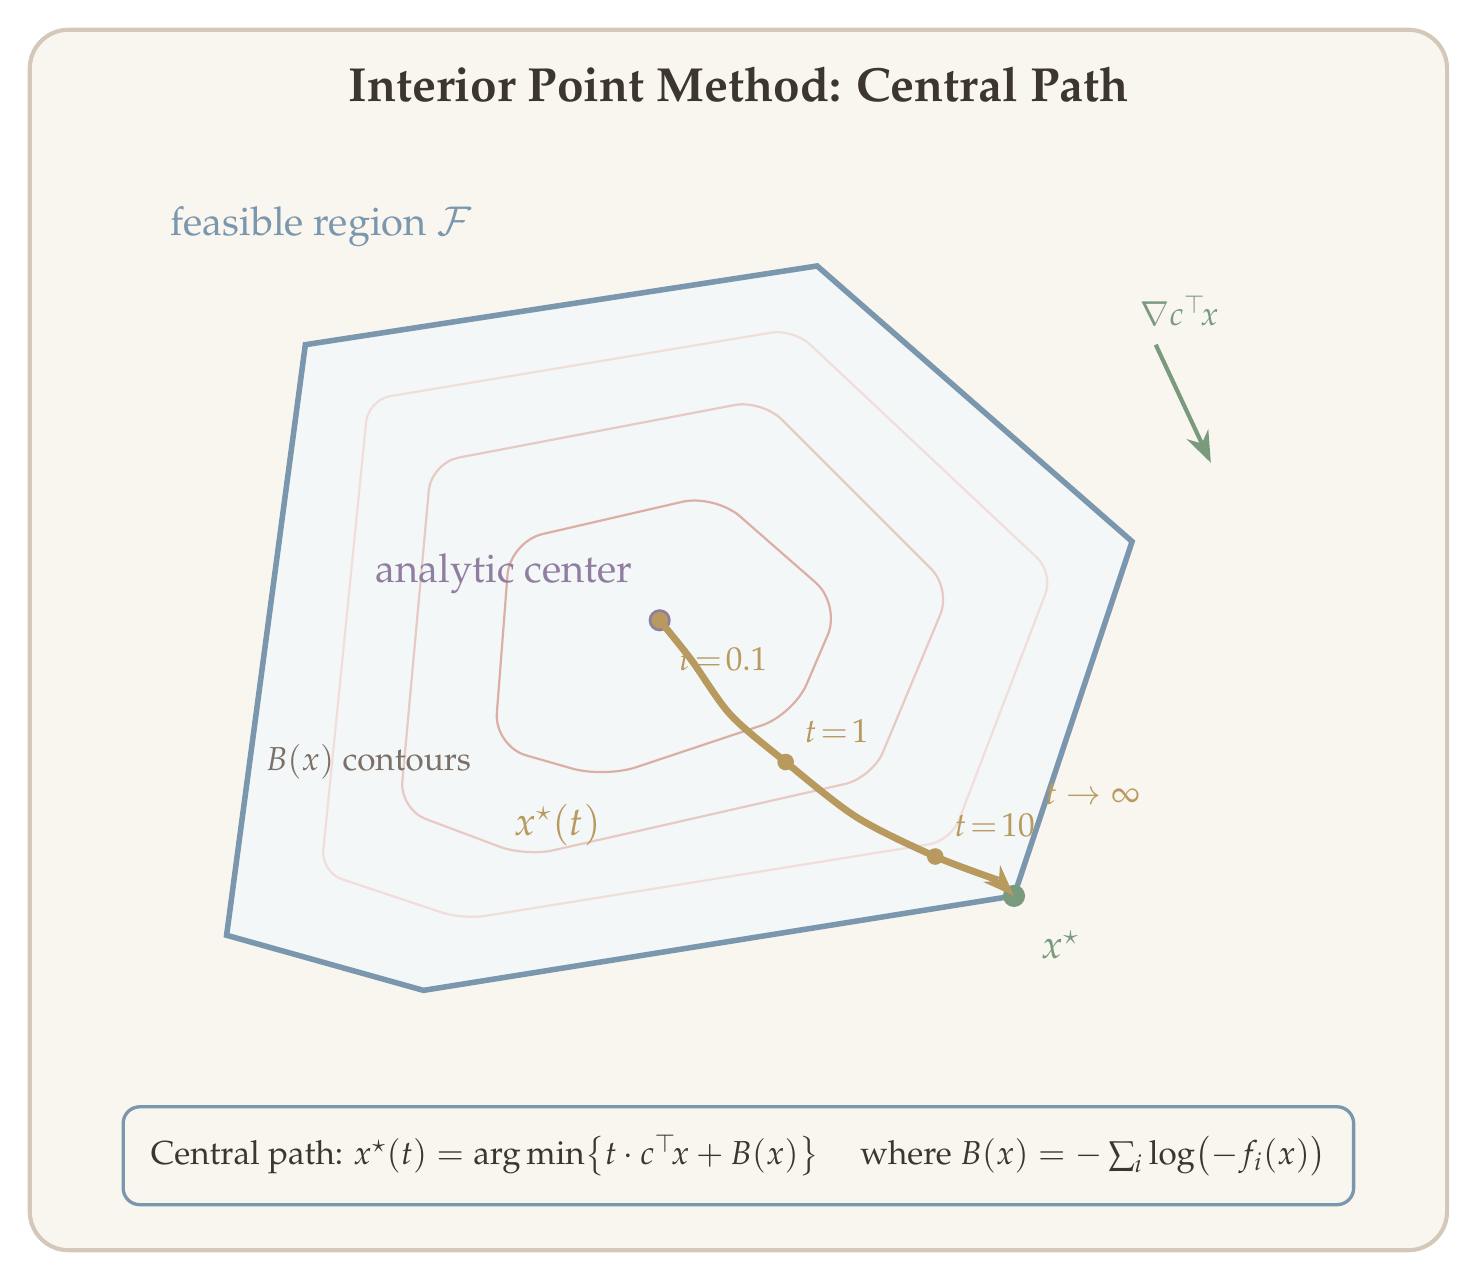
\begin{tikzpicture}[>={Stealth[length=4mm, width=3mm]}, line width=1.5pt]

% Background
\fill[cream, rounded corners=14pt] (-1.5,-3) rectangle (16.5,12.5);
\draw[border, line width=1.5pt, rounded corners=14pt] (-1.5,-3) rectangle (16.5,12.5);

% Title
\node[font=\LARGE\bfseries, text=dkbrown] at (7.5,11.8) {Interior Point Method: Central Path};

% Feasible region (polygon) - a pentagon-like region
\coordinate (P1) at (1,1);
\coordinate (P2) at (3.5,0.3);
\coordinate (P3) at (11,1.5);
\coordinate (P4) at (12.5,6);
\coordinate (P5) at (8.5,9.5);
\coordinate (P6) at (2,8.5);

% Barrier contours (draw BEFORE the polygon fill to get the layering right)
% Outer contour (near boundary) - faint
\draw[terracotta!25, line width=1pt, rounded corners=8pt]
  (2.2,1.8) -- (4,1.2) -- (10.2,2.2) -- (11.5,5.6) -- (8.2,8.7) -- (2.8,7.8) -- cycle;
% Middle contour
\draw[terracotta!40, line width=1pt, rounded corners=10pt]
  (3.2,2.6) -- (4.8,2.0) -- (9.2,3.0) -- (10.2,5.4) -- (7.8,7.8) -- (3.6,7.0) -- cycle;
% Inner contour
\draw[terracotta!60, line width=1pt, rounded corners=12pt]
  (4.4,3.4) -- (5.8,3.0) -- (8.2,3.8) -- (8.8,5.2) -- (7.2,6.6) -- (4.6,6.0) -- cycle;

% Feasible region outline
\fill[stblue!8] (P1) -- (P2) -- (P3) -- (P4) -- (P5) -- (P6) -- cycle;
\draw[stblue, line width=2pt] (P1) -- (P2) -- (P3) -- (P4) -- (P5) -- (P6) -- cycle;

% Redraw contours on top of fill
\draw[terracotta!25, line width=0.8pt, rounded corners=8pt]
  (2.2,1.8) -- (4,1.2) -- (10.2,2.2) -- (11.5,5.6) -- (8.2,8.7) -- (2.8,7.8) -- cycle;
\draw[terracotta!40, line width=0.8pt, rounded corners=10pt]
  (3.2,2.6) -- (4.8,2.0) -- (9.2,3.0) -- (10.2,5.4) -- (7.8,7.8) -- (3.6,7.0) -- cycle;
\draw[terracotta!60, line width=0.8pt, rounded corners=12pt]
  (4.4,3.4) -- (5.8,3.0) -- (8.2,3.8) -- (8.8,5.2) -- (7.2,6.6) -- (4.6,6.0) -- cycle;

\node[font=\large, text=wmgray] at (2.8,3.2) {$B(x)$ contours};

% Analytic center
\fill[lavender] (6.5,5.0) circle (4pt);
\node[font=\Large, text=lavender, above left] at (6.3,5.2) {analytic center};

% Optimal vertex (e.g., P3 area -- direction of optimization)
\node[font=\Large, text=sage, below right] at (11.2,1.2) {$x^\star$};
\fill[sage] (11,1.5) circle (4pt);

% Central path: curved from analytic center toward optimal vertex
\draw[rwgold, line width=2.5pt, smooth]
  plot coordinates {(6.5,5.0) (6.9,4.5) (7.4,3.8) (8.1,3.2) (9.0,2.5) (10.0,2.0) (10.8,1.7)};

% Points along the central path with t labels
\fill[rwgold] (6.5,5.0) circle (3pt);
\node[font=\large\bfseries, text=rwgold, below right] at (6.6,4.8) {$t\!=\!0.1$};

\fill[rwgold] (8.1,3.2) circle (3pt);
\node[font=\large\bfseries, text=rwgold, above right] at (8.2,3.3) {$t\!=\!1$};

\fill[rwgold] (10.0,2.0) circle (3pt);
\node[font=\large\bfseries, text=rwgold, above right] at (10.1,2.1) {$t\!=\!10$};

% Arrow suggesting t -> infinity
\draw[->, rwgold, line width=1.5pt, dashed] (10.8,1.7) -- (11,1.5);
\node[font=\large, text=rwgold] at (12.0,2.8) {$t \to \infty$};

% Central path label
\node[font=\Large\bfseries, text=rwgold] at (5.2,2.4) {$x^\star(t)$};

% Objective direction arrow
\draw[->, sage, line width=1.5pt] (12.8,8.5) -- (13.5,7.0);
\node[font=\large, text=sage, above] at (13.1,8.6) {$\nabla c^\top\! x$};

% Explanation boxes
\node[fill=cream, draw=stblue, line width=1.2pt, rounded corners=6pt,
      font=\large, text=dkbrown, align=left, inner sep=10pt]
  at (7.5,-1.8) {Central path: $x^\star(t) = \arg\min\bigl\{t \cdot c^\top\! x + B(x)\bigr\}$
  \quad where $B(x) = -\textstyle\sum_i \log\bigl(-f_i(x)\bigr)$};

% Feasible region label
\node[font=\Large, text=stblue] at (2.2,10.0) {feasible region $\mathcal{F}$};

\end{tikzpicture}
\end{document}
